% Présentation générale, technologie front back autres,
% README, markdown, Console
% https://en.wikipedia.org/wiki/Software_design#Design_considerations


\section{Introduction}
\label{sec:introduction}

\begin{frame}
    \frametitle{L'objectif du module}

    \begin{figure}
        \centering
        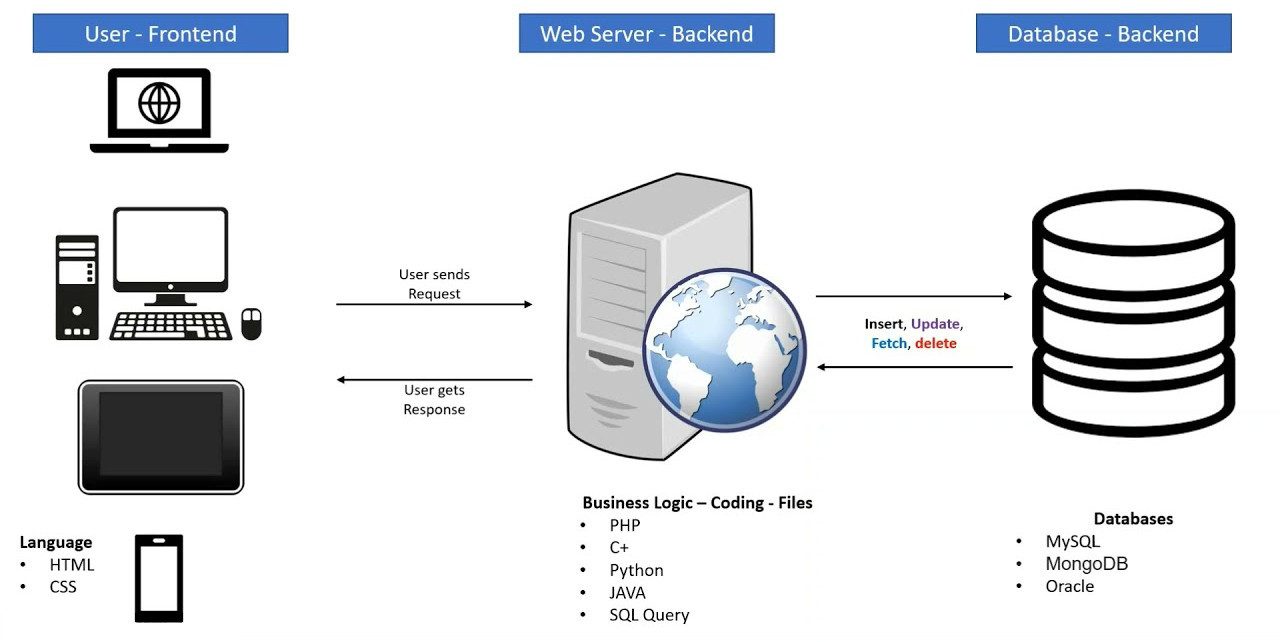
\includegraphics[width=\linewidth]{figures/introduction/overview}
        \label{fig:overview}
    \end{figure}
\end{frame}

\begin{frame}
    \frametitle{Le Web}

    \begin{figure}
        \centering
        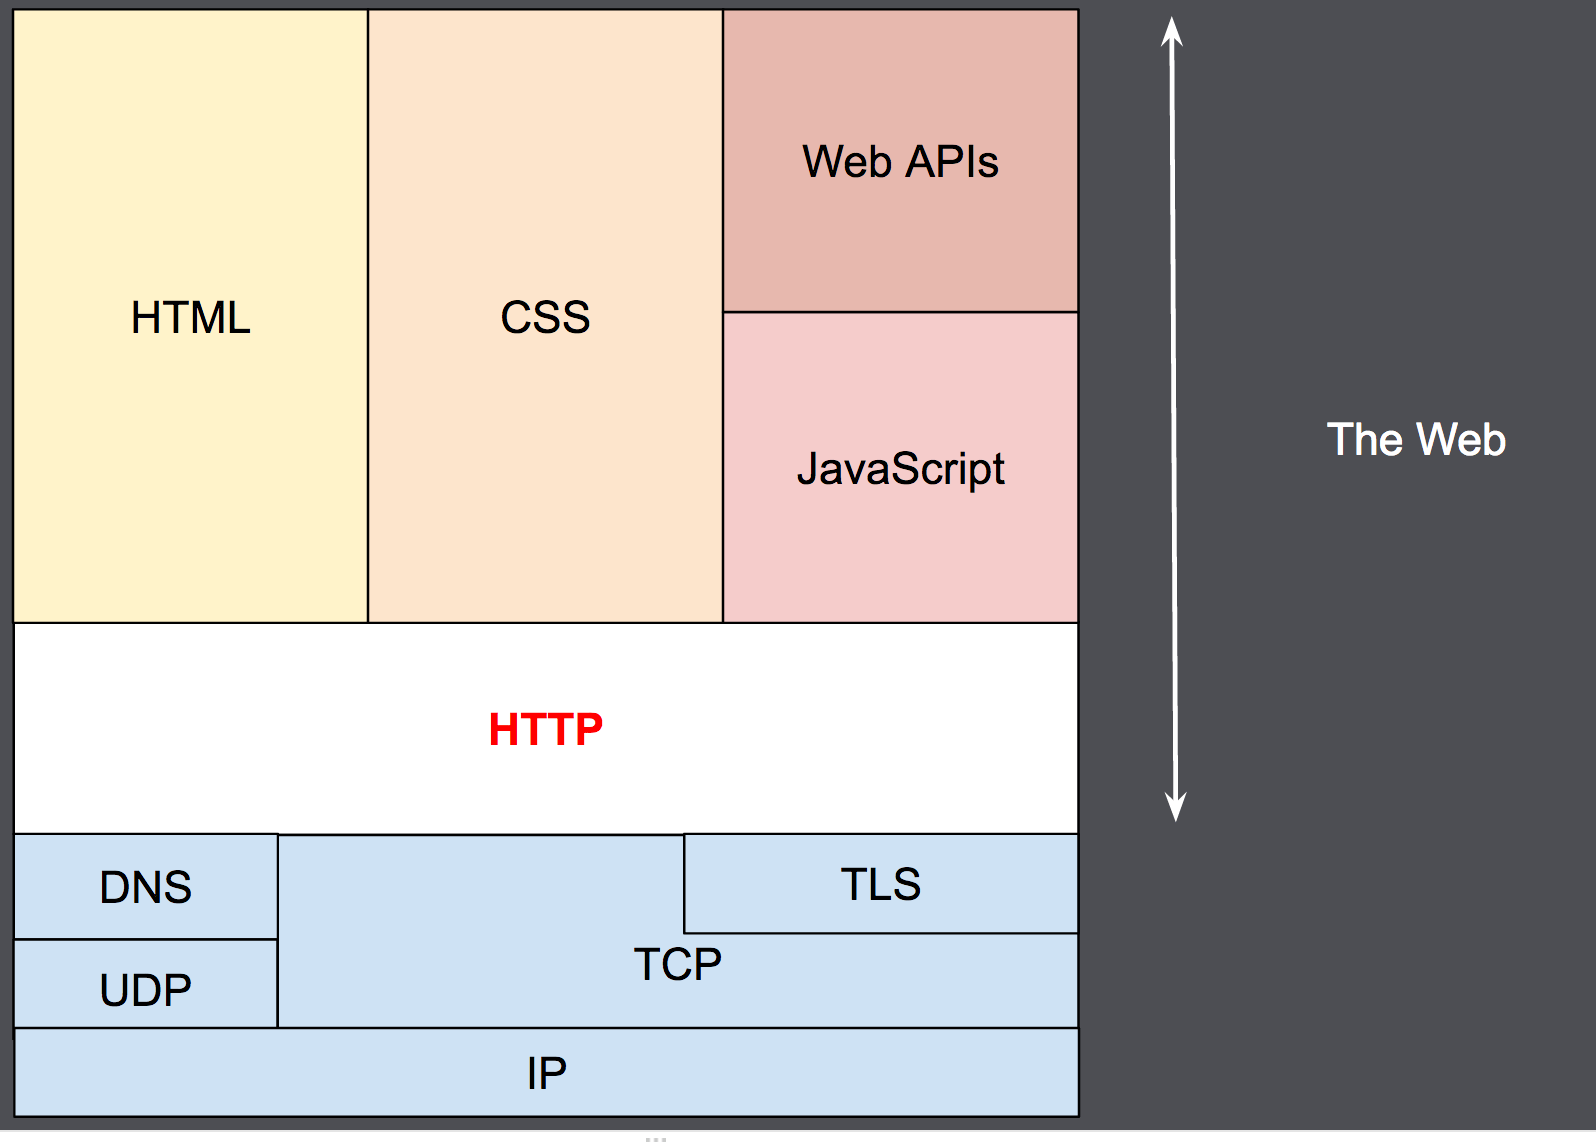
\includegraphics[height=0.5\linewidth]{figures/introduction/http-layers}
        \label{fig:web}
    \end{figure}
\end{frame}

\begin{frame}
    \frametitle{Le protocole HTTP}

    \begin{columns}
        \begin{column}{0.5\textwidth}
            \lstinputlisting[
                language=http,
                caption=Requête,
                label=lst:http-request]
            {figures/introduction/http-request.txt}
        \end{column}

        \begin{column}{0.5\textwidth}
            \lstinputlisting[
                language=http,
                caption=Réponse,
                label=lst:http-response]
            {figures/introduction/http-response.txt}
        \end{column}
    \end{columns}
\end{frame}

\begin{frame}
    \frametitle{Méthodes de requête HTTP}

    \begin{columns}
        \begin{column}{0.8\textwidth}
            HTTP définit un ensemble de méthodes (verbes) de requête qui indiquent l'action que l'on souhaite réaliser sur la ressource indiquée.
        \end{column}
        \begin{column}{0.2\textwidth}

            \qrcode[height=60pt]{https://developer.mozilla.org/fr/docs/Web/HTTP/Methods}
        \end{column}
    \end{columns}

    \begin{itemize}
        \item \textbf{GET} : demande une représentation de la ressource spécifiée, les requêtes GET doivent uniquement être utilisées afin de récupérer des données.
        \item \textbf{POST} : est utilisée pour envoyer une entité vers la ressource indiquée, cela entraîne généralement un changement d'état ou des effets de bord sur le serveur.
        \item \textbf{PUT} : remplace toutes les représentations actuelles de la ressource visée par le contenu de la requête.
        \item \textbf{DELETE} : supprime la ressource indiquée.
    \end{itemize}
\end{frame}

\begin{frame}
    \frametitle{Mon parcours}

    \begin{columns}
        \begin{column}{0.6\textwidth}
            \begin{itemize}
                \item 2020 : Doctorat sur la maintenabilité logicielle
                \item 2017 : Développeur \emph{Java}
                \item 2016 : Expert automatisation \emph{Cucumber}
                \item 2011 : Chef de projet testing
                \item 2008 : Testeur fonctionnel
                \item 2007 : Diplômé de l'ENSC
                \item 2004 : Licence d'électronique, électrotechnique et automatique
            \end{itemize}
        \end{column}

        \begin{column}{0.4\textwidth}
            \begin{figure}
                \centering
                \includesvg[width=0.8\textwidth]{figures/introduction/code-graph}
                \label{fig:code-graph}
            \end{figure}
        \end{column}
    \end{columns}
\end{frame}

\begin{frame}
    \frametitle{Le plan du module}

    \begin{columns}
        \begin{column}{0.6\textwidth}
            \begin{itemize}
                \item Modélisation UML
                \item L'environnement du développeur
                \item Les pratiques du développeur
                \item Les base de données
                \item La collaboration dans une équipe
                \item Les tests composants
                \item La contenerisation
                \item Le déploiement en continu
                \item Les patrons logiciels
                \item Le Document d'Architecture Technique
            \end{itemize}
        \end{column}

        \begin{column}{0.4\textwidth}
            \begin{itemize}
                \item WinForms
                \item UML
                \item Git et GitHub
                \item EFTodo
                \item EFUniversity
                \item MvcTodo
                \item MvcUniversity (2)
                \item Projet (3)
                \item TPDS
            \end{itemize}
        \end{column}
    \end{columns}
\end{frame}

\begin{frame}
    \frametitle{Architecture}

    \begin{figure}
        \centering
        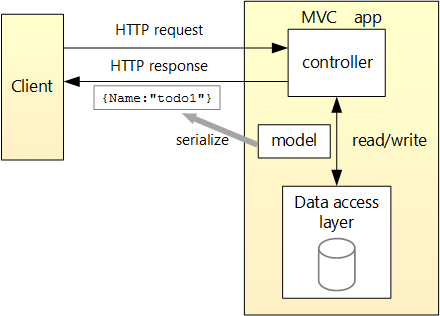
\includegraphics[height=0.5\linewidth]{figures/introduction/architecture}
        \label{fig:architexture}
    \end{figure}
\end{frame}



\begin{frame}
    \frametitle{Controlleur}

    \lstinputlisting[
        language={[Sharp]C},
        label=lst:controller]
    {figures/introduction/controller.cs}
\end{frame}


\begin{frame}
    \frametitle{DbContext}

    \lstinputlisting[
        language={[Sharp]C},
        label=lst:dbcontext]
    {figures/introduction/dbcontext.cs}
\end{frame}

\begin{frame}
    \frametitle{Les facettes du génie logiciel}

    \begin{columns}
        \begin{column}{0.4\textwidth}
            \begin{itemize}
                \item l'analyse fonctionnelle
                \item l'architecture
                \item la programmation
                \item les tests
                \item la maintenance
                \item la gestion de projet
                \item l'administration système
            \end{itemize}
        \end{column}
        \begin{column}{0.6\textwidth}
            \begin{figure}
                \centering
                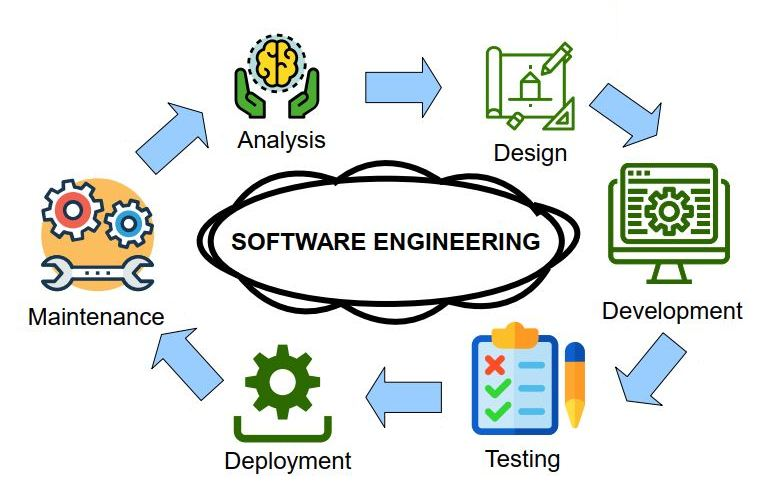
\includegraphics[width=\textwidth]{figures/introduction/software-engineering}
                \label{fig:engineering}
            \end{figure}
        \end{column}
    \end{columns}
\end{frame}

\begin{frame}
    \frametitle{Modélisation UML}

    \begin{figure}
        \centering
        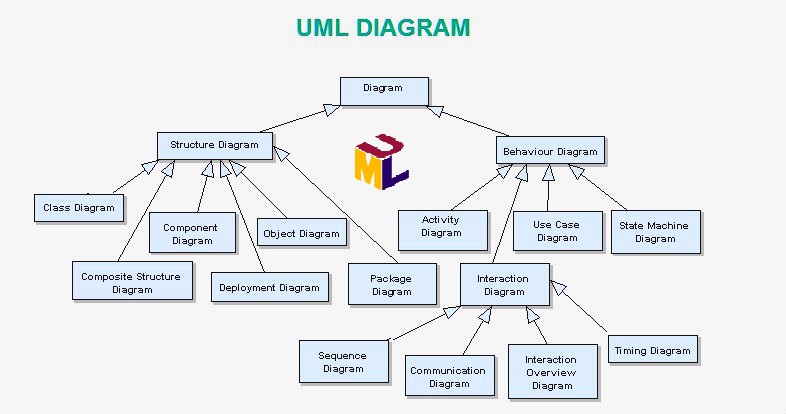
\includegraphics[height=0.5\linewidth]{figures/introduction/uml}
        \label{fig:uml}
    \end{figure}
\end{frame}

\begin{frame}
    \frametitle{L'environnement du développeur}

    \begin{figure}
        \centering
        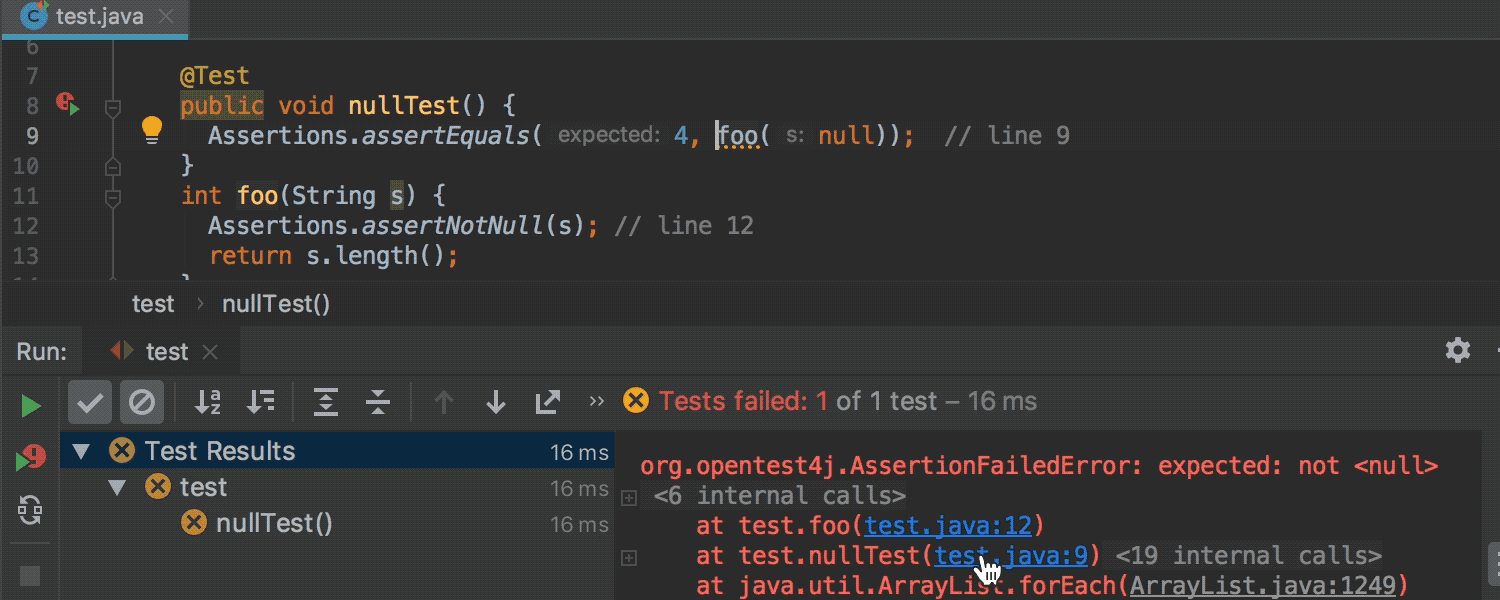
\includegraphics[width=\linewidth]{figures/introduction/intellij}
        \label{fig:environnement}
    \end{figure}
\end{frame}

\begin{frame}
    \frametitle{Les pratiques du développeur}

    \begin{figure}
        \centering
        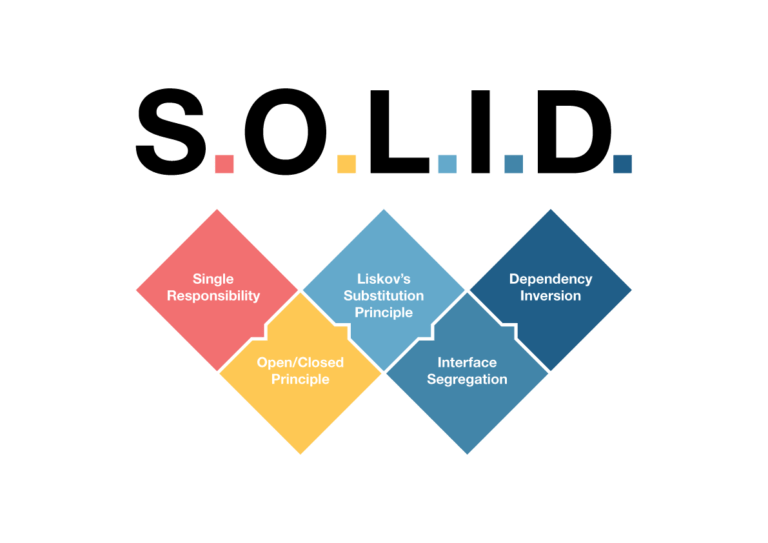
\includegraphics[height=0.5\linewidth]{figures/introduction/solid}
        \label{fig:pratiques}
    \end{figure}
\end{frame}

\begin{frame}
    \frametitle{Les base de données}

    \begin{figure}
        \centering
        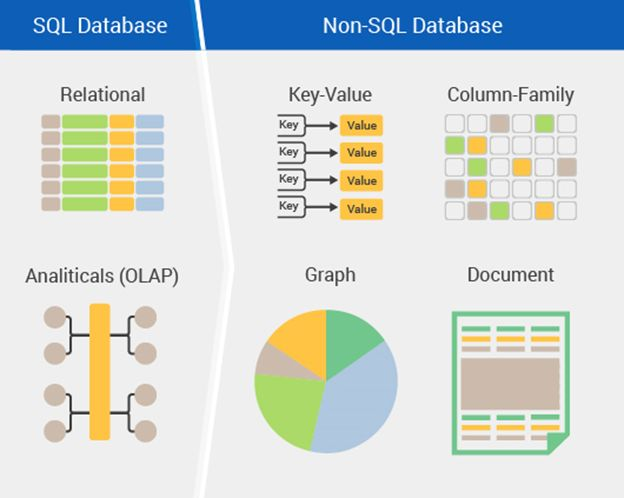
\includegraphics[height=0.5\linewidth]{figures/introduction/database}
        \label{fig:database}
    \end{figure}
\end{frame}

\begin{frame}
    \frametitle{La collaboration dans une équipe}

    \begin{figure}
        \centering
        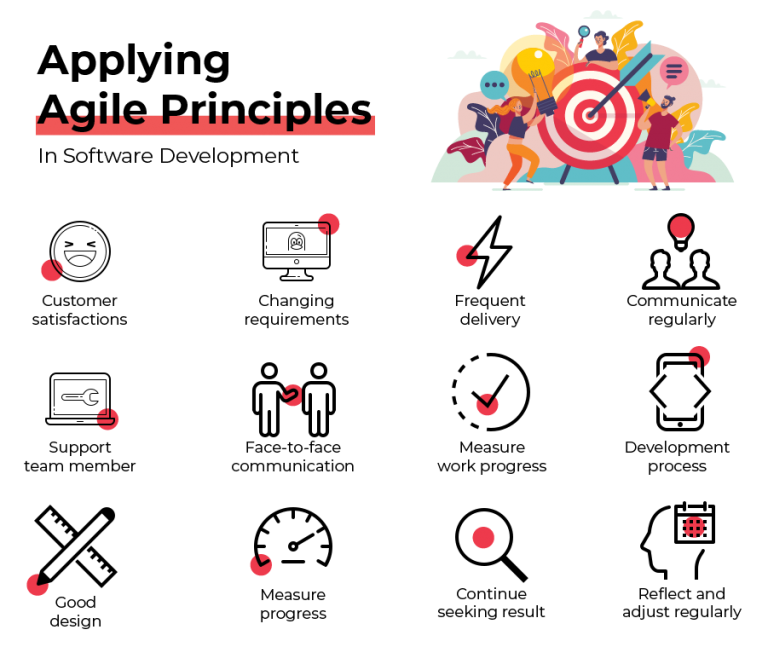
\includegraphics[height=0.5\linewidth]{figures/introduction/agile}
        \label{fig:collaboration}
    \end{figure}
\end{frame}

\begin{frame}
    \frametitle{Les tests composants}

    \begin{figure}
        \centering
        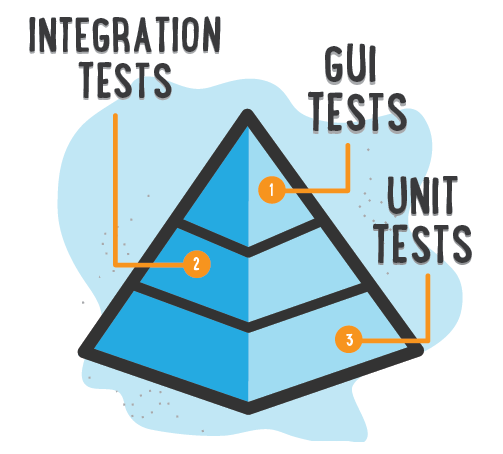
\includegraphics[height=0.5\linewidth]{figures/introduction/tests}
        \label{fig:tests}
    \end{figure}
\end{frame}

\begin{frame}
    \frametitle{La contenerisation}

    \begin{figure}
        \centering
        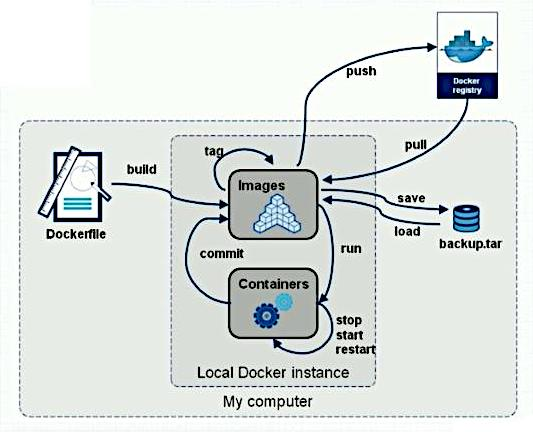
\includegraphics[height=0.5\linewidth]{figures/introduction/docker}
        \label{fig:conteneur}
    \end{figure}
\end{frame}

\begin{frame}
    \frametitle{Le déploiement en continu}

    \begin{figure}
        \centering
        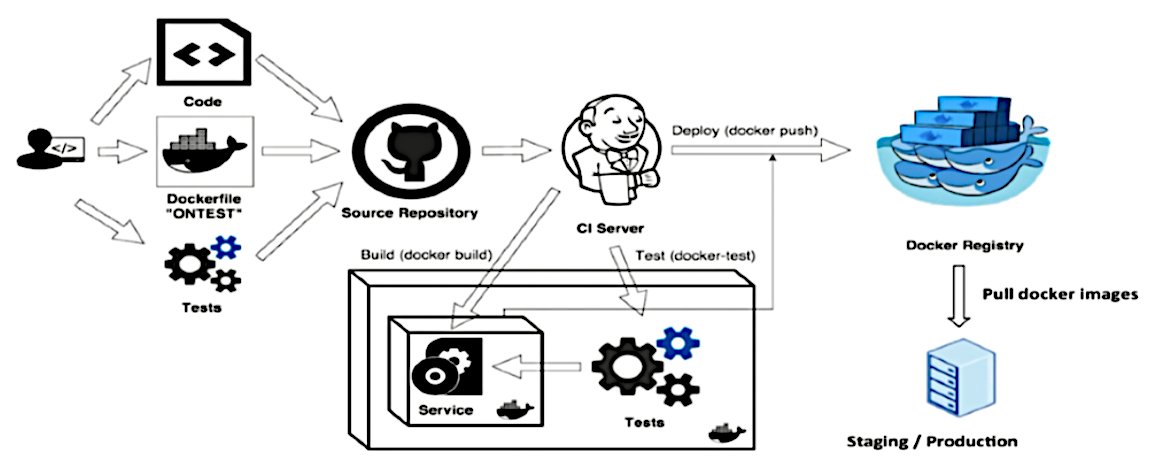
\includegraphics[width=\linewidth]{figures/introduction/continuous-deployment}
        \label{fig:deployment}
    \end{figure}
\end{frame}

\begin{frame}
    \frametitle{Les patrons logiciels}

    \begin{figure}
        \centering
        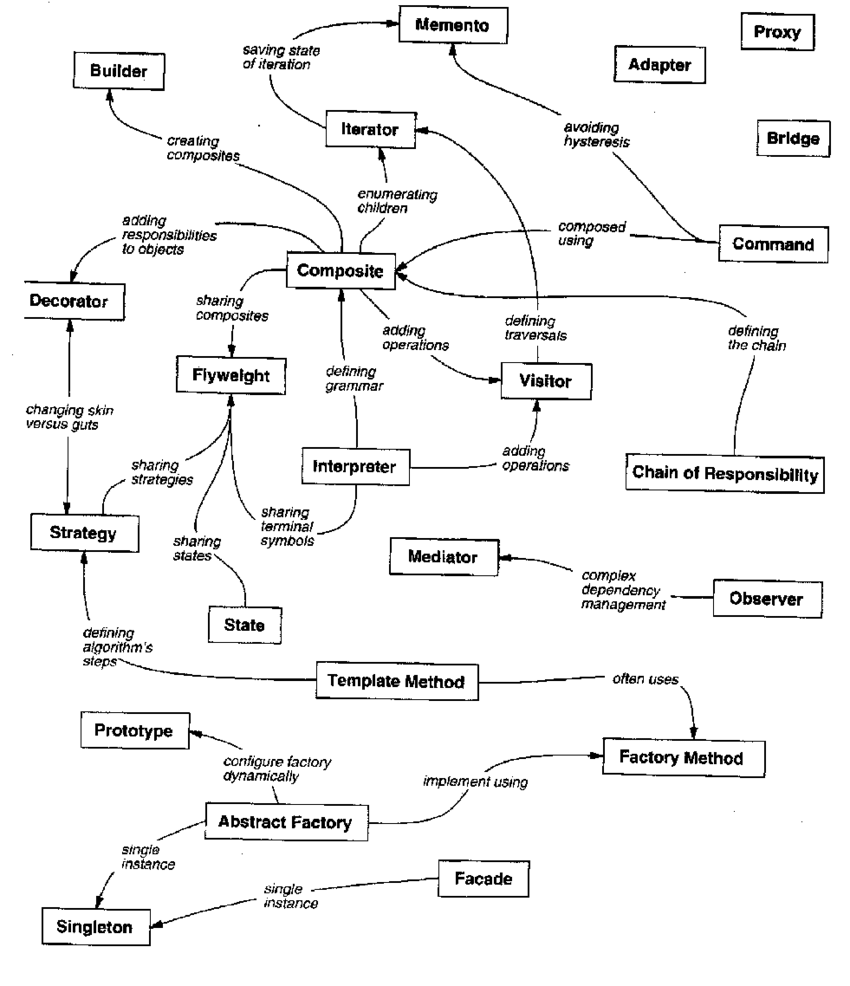
\includegraphics[height=0.5\linewidth]{figures/introduction/patrons}
        \label{fig:patrons}
    \end{figure}
\end{frame}

\begin{frame}
    \frametitle{Le Document d'Architecture Technique}

    \begin{figure}
        \centering
        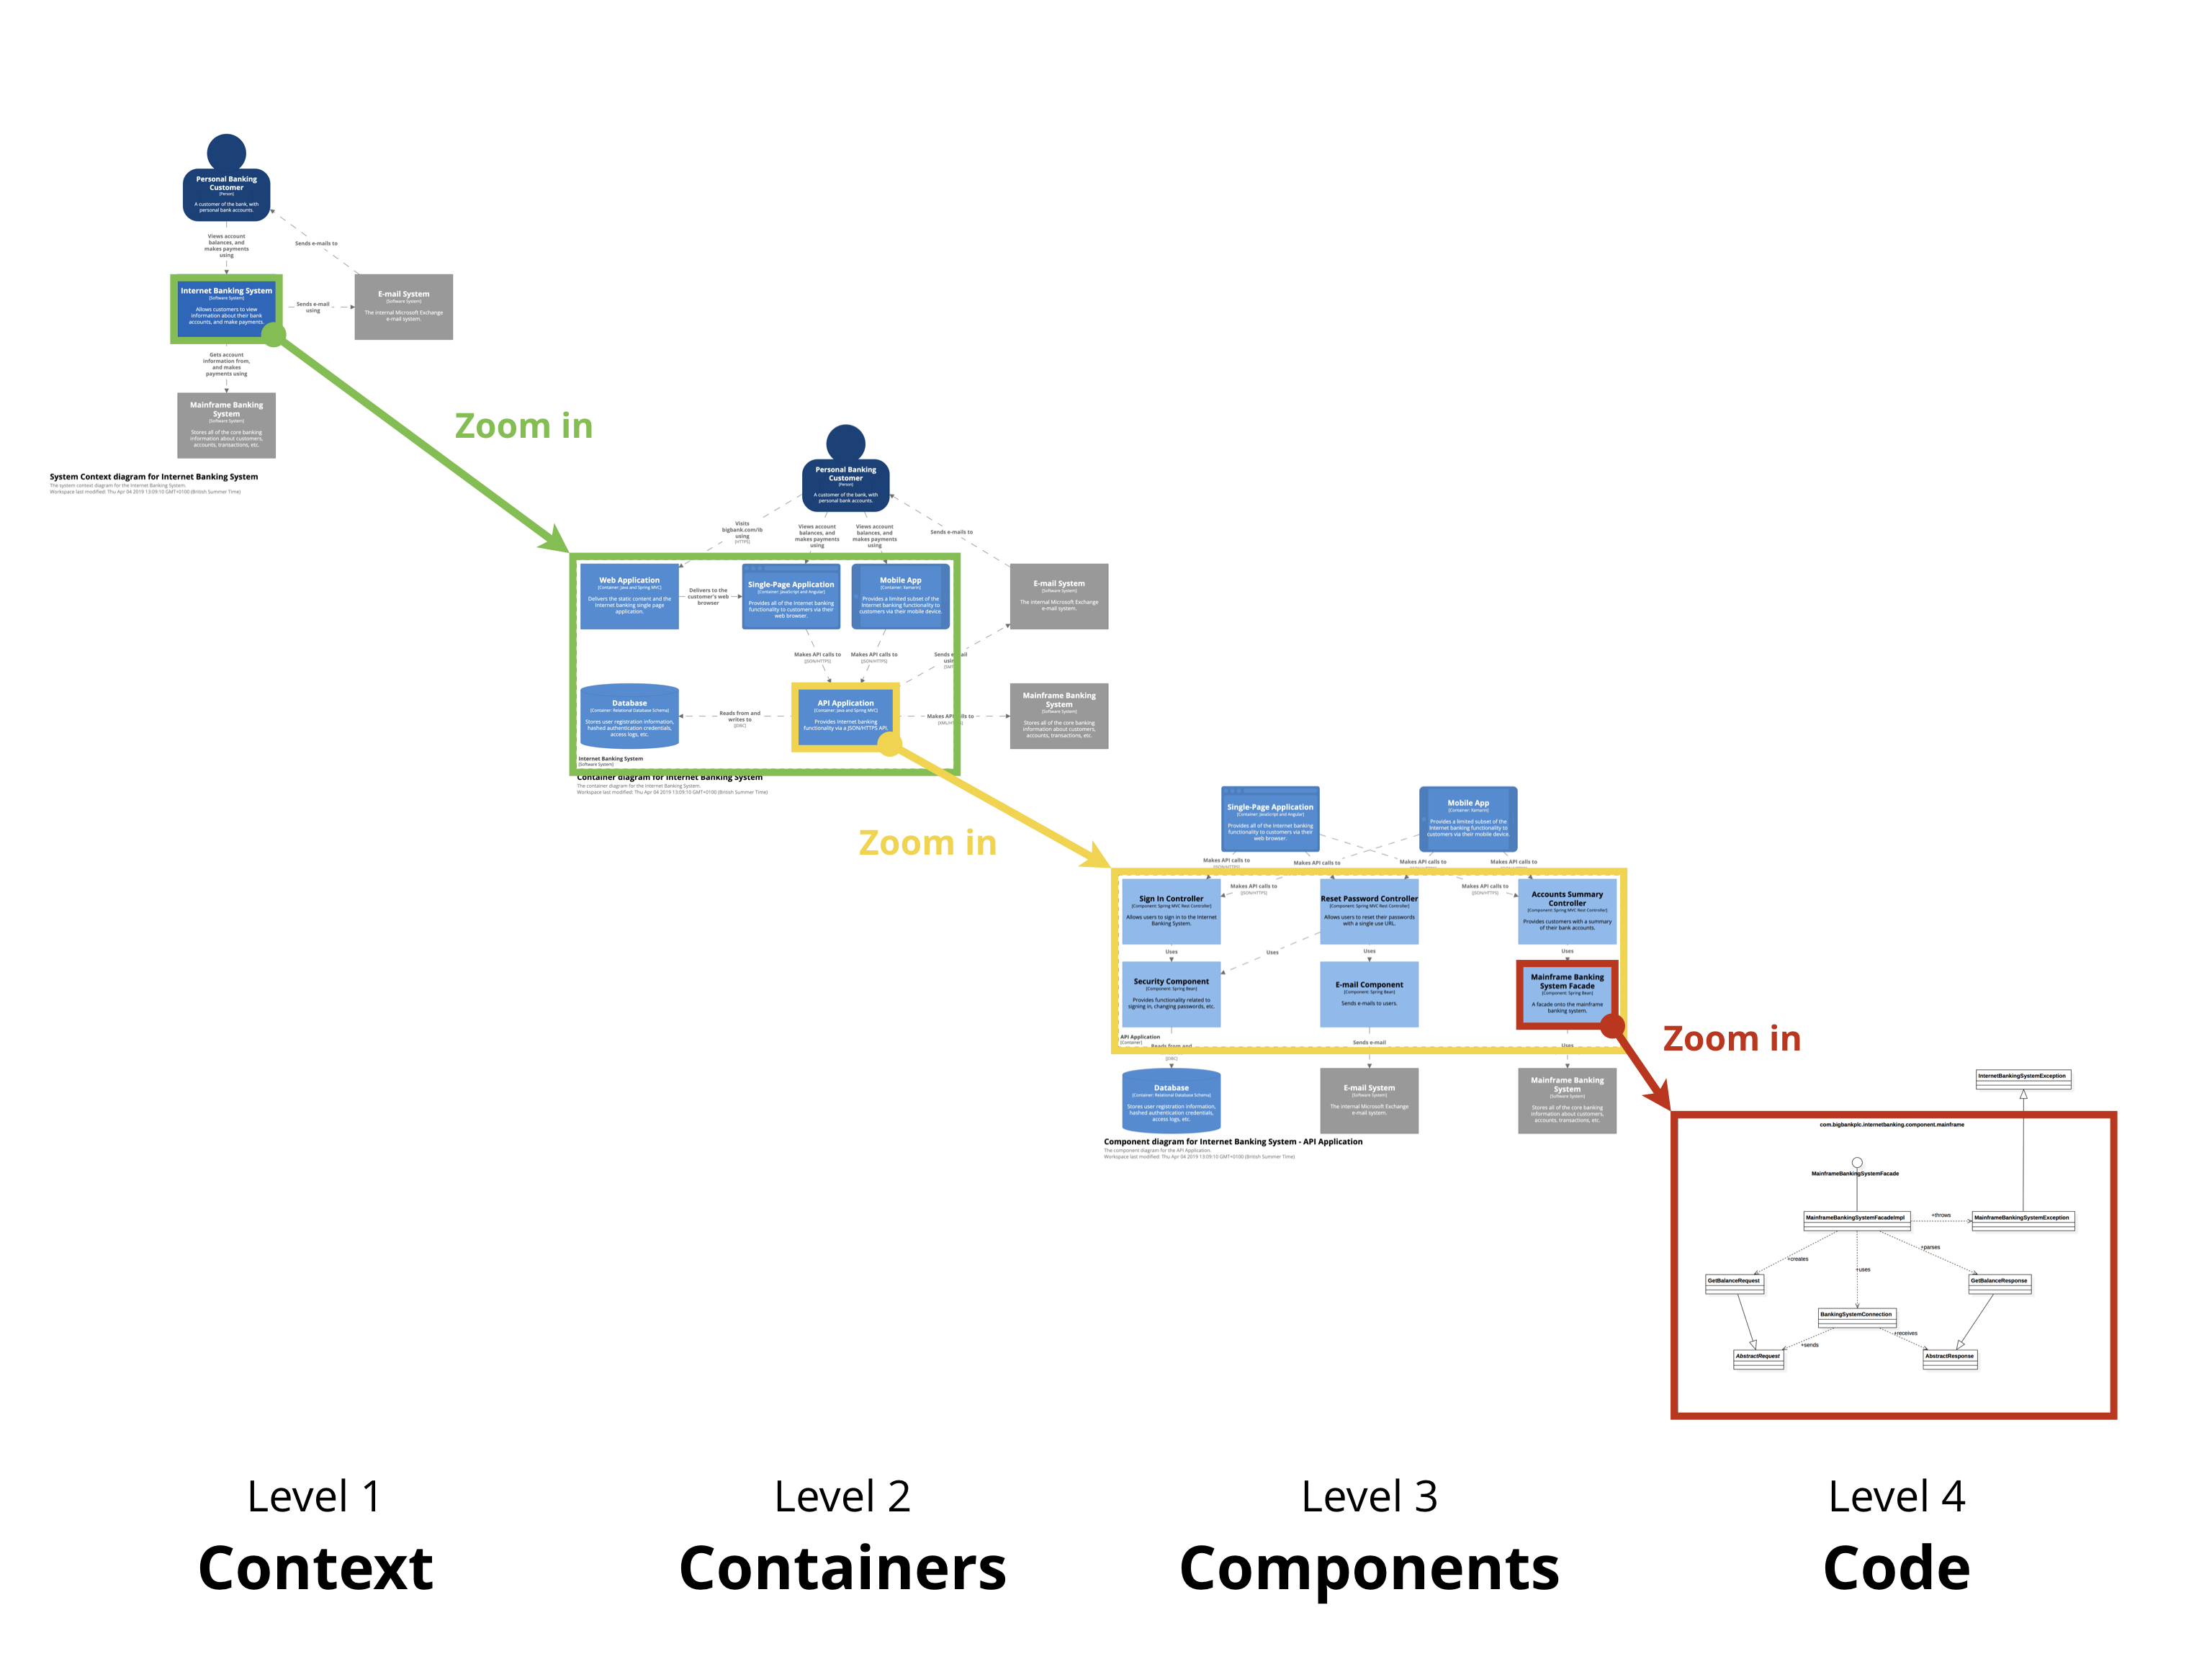
\includegraphics[height=0.5\linewidth]{figures/introduction/c4-overview}
        \label{fig:dat}
    \end{figure}
\end{frame}

\begin{frame}
    \frametitle{Deux livres de référence}
    \begin{columns}
        \begin{column}{0.5\textwidth}
            \begin{figure}
                \centering
                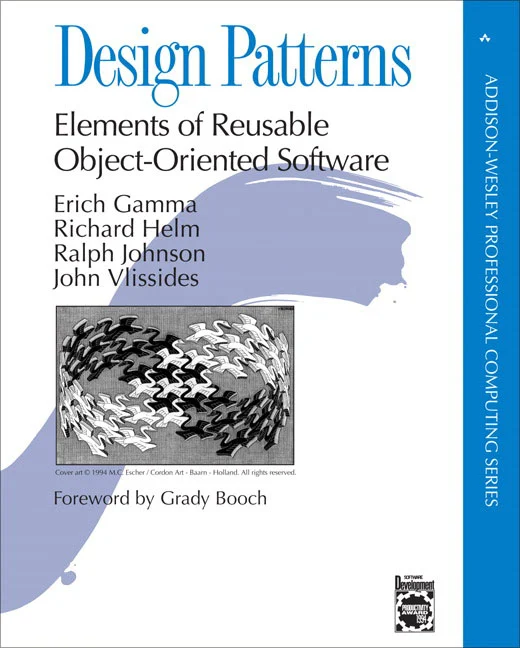
\includegraphics[height=\textwidth]{figures/introduction/book-design-patterns}
                \label{fig:book-design-patterns}
            \end{figure}
        \end{column}
        \begin{column}{0.5\textwidth}
            \begin{figure}
                \centering
                
\includegraphics[height=\textwidth]{figures/introduction/book-clean-code}
                \label{fig:book-clean-code}
            \end{figure}
        \end{column}
    \end{columns}
\end{frame}

\begin{frame}
    \frametitle{La méthode du canard en plastique}

    \begin{columns}
        \begin{column}{0.5\textwidth}
            \begin{figure}
                \centering
                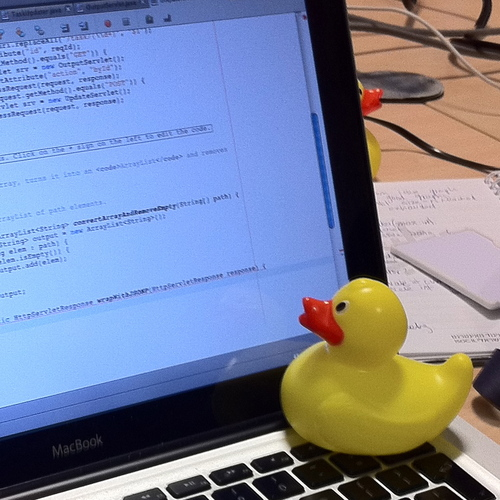
\includegraphics[height=\linewidth]{figures/introduction/canard}
                \label{fig:canard}
            \end{figure}
        \end{column}
        \begin{column}{0.5\textwidth}
            La méthode du canard en plastique consiste à expliquer méticuleusement le code source que l'on a écrit
            à un collègue, à un simple passant, ou même un canard en plastique.

            \bigskip
            L'avantage du canard en plastique sur un interlocuteur humain est que
            \emph{sa capacité d'écoute et sa patience sont sans limite}.
        \end{column}
    \end{columns}
\end{frame}
